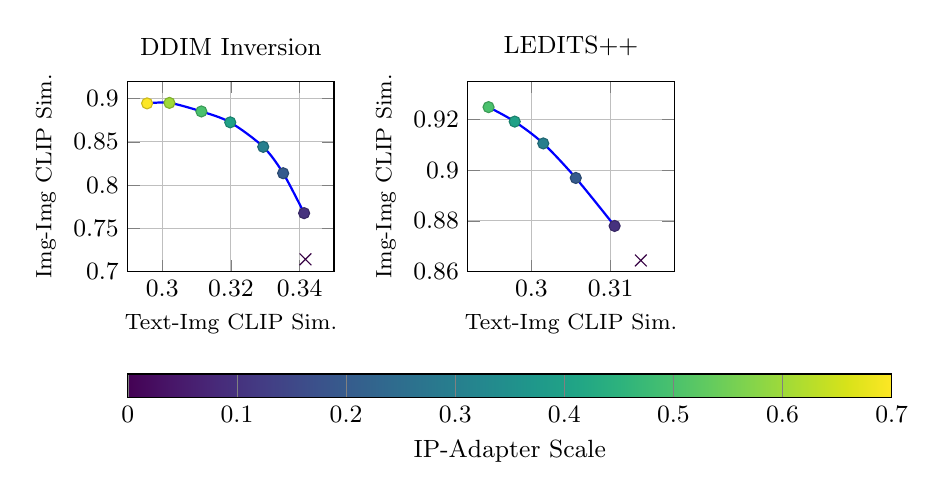
\begin{tikzpicture}
    \small{
    \begin{axis}[
        hide axis,
        scale only axis,
        height=0pt,
        colorbar horizontal,
        colormap/viridis, %
        colorbar style={
            width=0.8\linewidth, %
            height=0.3cm,
            yshift=-1cm,
            xlabel={IP-Adapter Scale}, %
            xticklabel style={/pgf/number format/.cd, fixed, precision=2},
        },
        point meta min=0.0, %
        point meta max=0.7, %
    ]
    \end{axis}

    \begin{axis}[
        name=plot1,
        width=4.2cm, height=4.0cm,
        xlabel={\footnotesize{Text-Img CLIP Sim.}},
        ylabel={\footnotesize{Img-Img CLIP Sim.}},
        title={DDIM Inversion},
        xmin=0.29, xmax=0.35,
        ymin=0.7, ymax=0.92,
        grid=both,
        legend pos=north west,
        colormap/viridis,
        colorbar=false, %
        point meta min=0.0, %
        point meta max=0.7, %
    ]
        \addplot[
            scatter,
            only marks,
            mark=*,
            mark size=2pt,
            scatter src=explicit, %
        ] table [meta=colormap] { %
            x       y       colormap
            0.3413  0.7676  0.1
            0.3352  0.8137  0.2
            0.3294  0.8442  0.3
            0.3198  0.8725  0.4
            0.3114  0.8851  0.5
            0.3021  0.8950  0.6
            0.2956  0.8944  0.7
        };

        \addplot[
            scatter,
            only marks,
            mark=x, %
            mark size=3pt, %
            scatter src=explicit,
        ] table [meta=colormap] {
            x       y       colormap
            0.3417  0.7143  0.0
        };
        
        \addplot[
            smooth,
            thick,
            blue,
        ] table {
            x       y
            0.3413  0.7676
            0.3352  0.8137
            0.3294  0.8442
            0.3198  0.8725
            0.3114  0.8851
            0.3021  0.8950
            0.2956  0.8944
        };
    \end{axis}

    \hspace{8pt}
    \begin{axis}[
        name=plot2,
        at=(plot1.right of south east), anchor=left of south west,
        width=4.2cm, height=4.0cm,
        xlabel={\footnotesize{Text-Img CLIP Sim.}},
        ylabel={\footnotesize{Img-Img CLIP Sim.}},
        title={LEDITS++},
        xmin=0.292, xmax=0.318,
        ymin=0.86, ymax=0.935,
        grid=both,
        legend pos=north west,
        colormap/viridis,
        colorbar=false, %
        point meta min=0.0, %
        point meta max=0.7, %
    ]
        \addplot[
            scatter,
            only marks,
            mark=*,
            mark size=2pt,
            scatter src=explicit, %
        ] table [meta=colormap] { %
            x       y       colormap
            0.3105  0.8780  0.1
            0.3056  0.8969  0.2
            0.3015  0.9105  0.3
            0.2979  0.9191  0.4
            0.2946  0.9248  0.5
        };

        \addplot[
            scatter,
            only marks,
            mark=x, %
            mark size=3pt, %
            scatter src=explicit,
        ] table [meta=colormap] {
            x       y       colormap
            0.3138  0.8644  0.0
        };
        
        \addplot[
            smooth,
            thick,
            blue,
        ] table {
            x       y
            0.3105  0.8780
            0.3056  0.8969
            0.3015  0.9105
            0.2979  0.9191
            0.2946  0.9248
        };
    \end{axis}
    }
\end{tikzpicture}
